\documentclass[10pt,a4paper]{article}
\usepackage[margin=1.5cm]{geometry}
\usepackage{graphicx}
\usepackage{subcaption}
\usepackage{booktabs}
\usepackage{titlesec}
\setlength{\parindent}{0pt}
\setlength{\parskip}{3pt}
\titlespacing*{\section}{0pt}{7pt}{3pt}

\begin{document}

\begin{center}
{\large Machine Learning -- Exercise 0: Dataset Description}\\[5pt]
Group 66\\[3pt]
Aaradhaya Arora (12534787)\\
Serhii Slutu (12537831)\\
Paul H\"ubner (00371292)
\end{center}

\vspace{-5pt}

\section{The Datasets}
The Cylinder Bands dataset is about problems in a printing process. The data contains information about the printing materials, machines and process settings. There are 540 observations and 39 input attributes.

The Page Blocks dataset is about different areas of document pages. Each observation describes one block of a page, with measurements such as its height, length, area and pixel information. There are 5,473 observations and 10 input attributes.

\section{Why We Chose Them}
We chose these two datasets from OpenML because they differ in several ways. Page Blocks has about ten times as many observations as Cylinder Bands, but fewer input attributes. Cylinder Bands has numerical and categorical inputs, while Page Blocks has only numerical inputs. They also differ in their target classes, missing values and class distributions.

\begin{center}
\begin{tabular}{lcc}
\toprule
 & Cylinder Bands & Page Blocks \\
\midrule
Observations & 540 & 5,473 \\
Input attributes & 39 & 10 \\
Target classes & 2 & 5 \\
Input types & Numerical and categorical & Numerical \\
Missing values & Yes & No \\
\bottomrule
\end{tabular}
\end{center}

\section{Target Classes}
Cylinder Bands has two classes: band means that a printing problem called cylinder banding occurs, while noband means that it does not occur. The classes are quite evenly distributed, with 42.2\% band and 57.8\% noband.

Page Blocks has five classes: text (1), horizontal line (2), picture (3), vertical line (4) and graphic (5). Almost 90\% of the observations are text blocks. The other four classes are much smaller, with only 28 observations in the smallest class. This is important because predicting the most common class would already result in a high accuracy, even if the other classes were not predicted correctly.

\begin{figure}[h!]
\centering
\begin{subfigure}{0.49\textwidth}
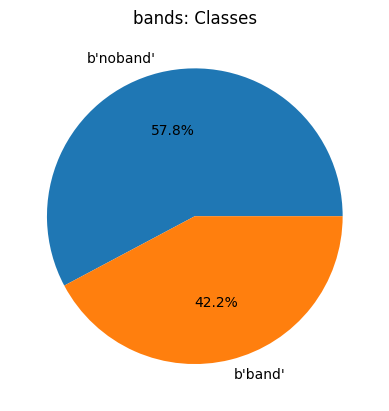
\includegraphics[width=\linewidth,height=5.0cm,keepaspectratio]{figures/bands_classes.png}
\caption{Cylinder Bands}
\end{subfigure}\hfill
\begin{subfigure}{0.49\textwidth}
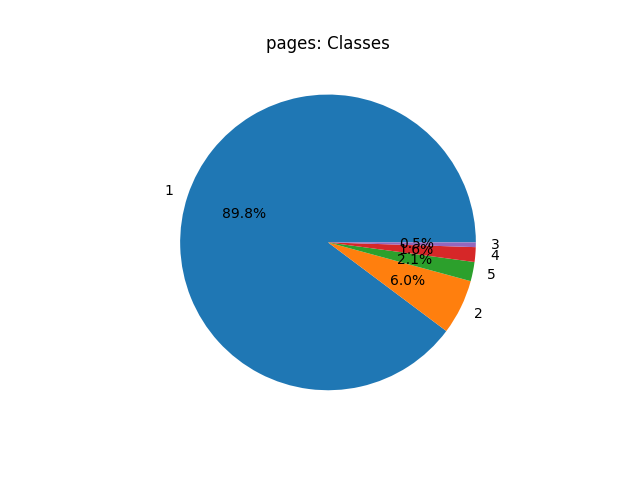
\includegraphics[width=\linewidth,height=5.0cm,keepaspectratio]{figures/pages_classes.png}
\caption{Page Blocks}
\end{subfigure}
\caption{Target class distributions.}
\end{figure}

\newpage
\section{Missing Values}
Cylinder Bands has missing values in 28 of its 39 input attributes. The attribute \texttt{paper\_mill\_location} has the most missing values, with 156 out of 540 observations (28.9\%). Before training a model, missing numerical values could be replaced by the median, and missing categorical values by the most common category. Page Blocks has no missing values.

\begin{figure}[h!]
\centering
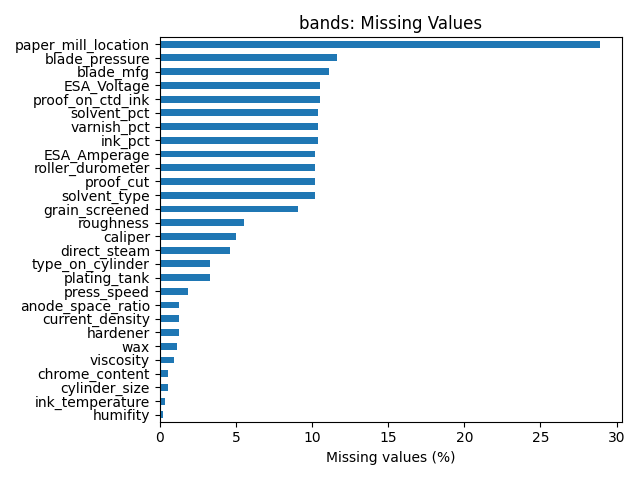
\includegraphics[width=0.95\textwidth,height=5.7cm,keepaspectratio]{figures/bands_missing.png}
\caption{Missing values by attribute in Cylinder Bands.}
\end{figure}

\section{Numerical Attributes and Preprocessing}
The numerical attributes have very different ranges. In Cylinder Bands, \texttt{press\_speed} ranges from 0 to 2,600, while \texttt{roughness} ranges from about 0.06 to 1.25. In Page Blocks, \texttt{area} ranges from 7 to 143,993, while \texttt{p\_black} ranges from about 0.05 to 1. Some attributes also have a few values that are much higher than most of the others.

Scaling numerical values could therefore be useful for both datasets. Cylinder Bands also contains categorical inputs that may need to be converted before using some classification methods. Columns used only as identifiers, such as cylinder number, should also be considered separately.

\begin{figure}[h!]
\centering
\begin{subfigure}{0.49\textwidth}
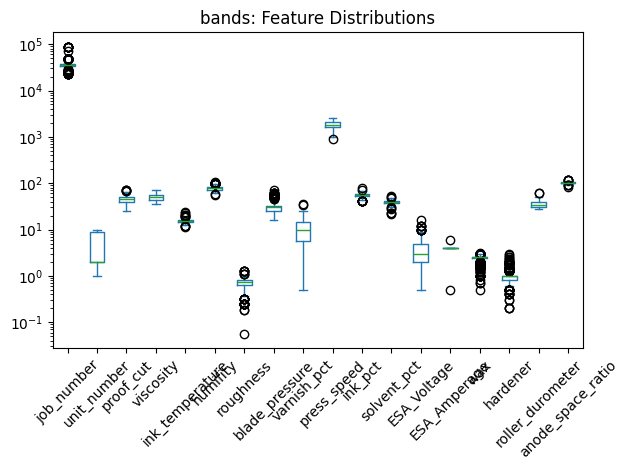
\includegraphics[width=\linewidth,height=5.3cm,keepaspectratio]{figures/bands_boxplot.png}
\caption{Cylinder Bands}
\end{subfigure}\hfill
\begin{subfigure}{0.49\textwidth}
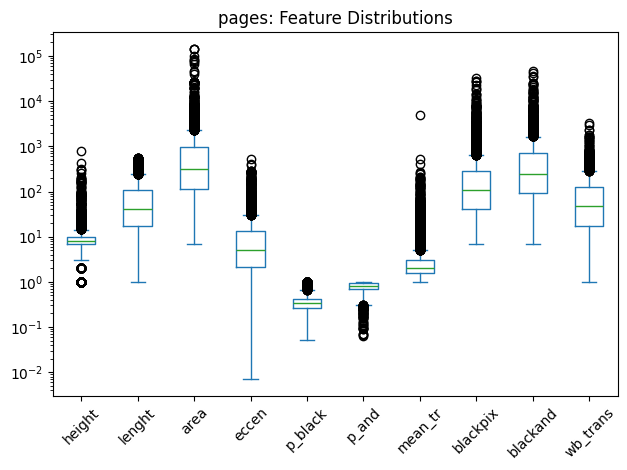
\includegraphics[width=\linewidth,height=5.3cm,keepaspectratio]{figures/pages_boxplot.png}
\caption{Page Blocks}
\end{subfigure}
\caption{Numerical values on a logarithmic scale. Zero values are not shown.}
\end{figure}
\end{document}
